\documentclass[12pt,letterpaper]{article}
\usepackage[utf8]{inputenc}
\usepackage{tikz}
\usetikzlibrary{trees}
\usepackage[spanish, es-nodecimaldot]{babel}
\usepackage{amsmath}
\usepackage{color}
\usepackage{algorithm}
\usepackage[noend]{algpseudocode}
\renewcommand{\algorithmicrequire}{\textbf{Entrada:}}
\renewcommand{\algorithmicensure}{\textbf{Salida:}}
\usepackage{subcaption}
\usepackage{amsfonts}
\usepackage{hyperref}
 \hypersetup{
     colorlinks=true,
     linkcolor=blue,
     filecolor=blue,
     citecolor = blue,      
     urlcolor=cyan,
     }
\usepackage{amssymb}
\usepackage{listings}
\usepackage{color}

\definecolor{mygreen}{rgb}{0,0.6,0}
\definecolor{mygray}{rgb}{0.5,0.5,0.5}
\definecolor{mymauve}{rgb}{0.58,0,0.82}

\lstset{ 
  backgroundcolor=\color{white},   % choose the background color; you must add \usepackage{color} or \usepackage{xcolor}; should come as last argument
  basicstyle=\footnotesize,        % the size of the fonts that are used for the code
  breakatwhitespace=false,         % sets if automatic breaks should only happen at whitespace
  breaklines=true,                 % sets automatic line breaking
  captionpos=b,                    % sets the caption-position to bottom
  commentstyle=\color{mygreen},    % comment style
  deletekeywords={...},            % if you want to delete keywords from the given language
  escapeinside={\%*}{*)},          % if you want to add LaTeX within your code
  extendedchars=true,              % lets you use non-ASCII characters; for 8-bits encodings only, does not work with UTF-8
  firstnumber=1,                % start line enumeration with line 1000
  frame=single,	                   % adds a frame around the code
  keepspaces=true,                 % keeps spaces in text, useful for keeping indentation of code (possibly needs columns=flexible)
  keywordstyle=\color{blue},       % keyword style
  language=R,                 % the language of the code
  morekeywords={*,...},            % if you want to add more keywords to the set
  numbers=none,                    % where to put the line-numbers; possible values are (none, left, right)
  numbersep=5pt,                   % how far the line-numbers are from the code
  numberstyle=\tiny\color{mygray}, % the style that is used for the line-numbers
  rulecolor=\color{black},         % if not set, the frame-color may be changed on line-breaks within not-black text (e.g. comments (green here))
  showspaces=false,                % show spaces everywhere adding particular underscores; it overrides 'showstringspaces'
  showstringspaces=false,          % underline spaces within strings only
  showtabs=false,                  % show tabs within strings adding particular underscores
  stepnumber=2,                    % the step between two line-numbers. If it's 1, each line will be numbered
  stringstyle=\color{mymauve},     % string literal style
  tabsize=2,	                   % sets default tabsize to 2 spaces
  title=\lstname                   % show the filename of files included with \lstinputlisting; also try caption instead of title
}

\usepackage{amsthm}
\newtheorem{theorem}{Teorema}

\usepackage{graphicx}
\usepackage[inner=1.5 cm, outer = 1.5 cm, top=1 cm, bottom = 1.5 cm]{geometry}
\setlength{\parskip}{3mm}
\title{\textsc{Valor esperado y varianza \\ Ejercicios \\ Simulación}}
\author{\textsc{Fabiola Vázquez}}

\setlength{\parindent}{0cm}
\renewcommand{\lstlistingname}{Código}
\floatname{algorithm}{Algoritmo}
\newtheorem{ej}{Ejercicio}

\begin{document}
\maketitle
\hrule
\section{Introducción}
En la tarea anterior \cite{fab} fueron realizados diversos ejercicios del libro de Grinstead y Snell \cite{snell}. El objetivo de este trabajo es realizar una simulación de algunos de estos ejercicios, dicha simulación se realiza con el software R \cite{R} en un cuaderno de Jupyter \cite{jupyter}.
\section{Ejercicios}

\begin{ej}[Ej. 1, p. 247] 
Se saca una carta al azar de una baraja que consiste de cartas numeradas del 2 al 10. Un jugador gana un dólar si el número en la carta es impar y pierde un dólar si el número es par. ¿Cuál es el valor esperado de sus ganancias?.
\end{ej}
\begin{proof}[Simulación]
Se considera la variable \texttt{carta} como un valor entre 2 y 10 y se verifica si dicho valor es divisible entre dos y se le asigna una ganancia de -1, en caso contrario se asigna una ganancia de 1. El proceso se repite una cantidad \texttt{t} de veces para calcular la media y ver si se aproxima al valor esperado, esto se automatiza con la función \texttt{cartas\_funcion}.
\begin{lstlisting}
cartas_funcion <- function(t){
    m <- c()
    for (j in 1:t){
		carta<-sample(x = 2:10,size = 1)
        if(carta%%  2==0){
            ganancia <- -1
        } else{ganancia <-1}
        m[j] <- ganancia
    }
return(mean(m))   
}
\end{lstlisting}
El experimento se corre variando \texttt{t} en $\{10, 100, 1000, 10000, 100000, 1000000\}$ y para cada uno de los valores se replica 100 veces. En la figura \ref{ej1} se muestra los gráficos de caja con los datos recopilados, la recta horizontal roja está ubicada en el valor $-\frac{1}{9}$, el cual es el valor encontrado analíticamente. Como se aprecia en dicha gráfica, entre mayor es el valor de \texttt{t} la media se aproxima al valor de $-\frac{1}{9}$.
\begin{figure}
 	\centering 
 		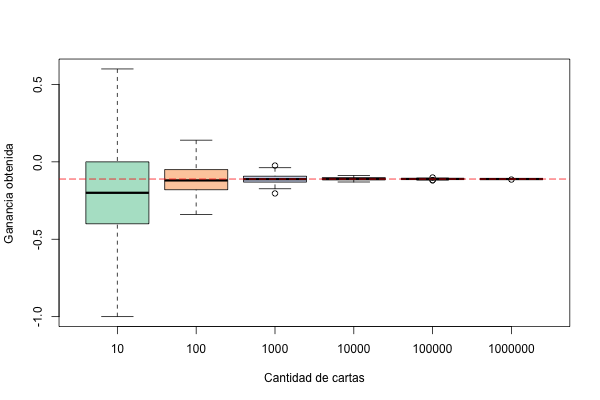
\includegraphics[scale=0.6]{ej1.png} 		
 	 	\caption{Gráficas de caja con las medias del ejercicio 1.} 
 	 		\label{ej1}
\end{figure}

\end{proof}

\begin{ej}[Ej. 6, p.247]
Se lanza un dado dos veces. Sea $X$ la suma de los dos números que aparecen, y sea $Y$ la diferencia de los números (específicamente, el número que aparece primera tirada menos el número de la segunda). Demuestra que $E(XY)=E(X)E(Y).$ ¿Son $X$ e $Y$ independientes?.
\end{ej}
\begin{proof}[Simulación] 
Primero, se va a estimar el valor esperado de la variable $X$, para ello se definen dos variables \texttt{dado1} y \texttt{dado2} como un valor pseudo aleatorio entre 1 y 6, y la variable \texttt{dado} se define como la suma de los otros dos. Se repite una cantidad \texttt{t} de veces para calcular la media y ver si se aproxima al valor esperado, esto se automatiza con la función \texttt{dados\_funcion}.
\begin{lstlisting}
dado_funcion <- function(n){
    m <- c()
    for (j in 1:n){
    dado1 <- sample(x = 1:6,size = 1,replace = TRUE)
    dado2 <- sample(x = 1:6,size = 1,replace = TRUE)
    dado <- dado1+dado2
    m[j] <- dado
    }
return(mean(m))
}
\end{lstlisting}
Al igual que el experimento anterior, este se corre variando \texttt{t} en $\{10, 100, 1000, 10000, 100000, 1000000\}$ y para cada uno de los valores se replica 100 veces. La figura \ref{ej2a} muestra los gráficos de caja con los datos obtenidos, la recta roja está ubicada en el valor 7, el cual es el valor de $E(X)$, encontrado analíticamente. Como se aprecia en dicha gráfica, entre mayor es el valor de \texttt{t} la media se aproxima al valor esperado encontrado.
\begin{figure}
 	\centering 
 		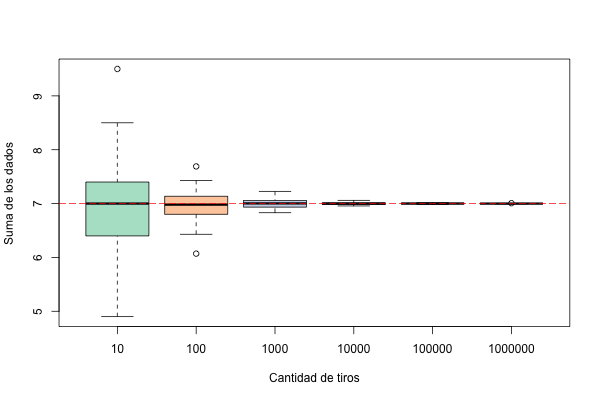
\includegraphics[scale=0.6]{ej2a.png} 		
 	 	\caption{Gráficas de caja con las medias de la suma de dados del ejercicio 2.} 
 	 		\label{ej2a}
\end{figure}
Similarmente, se estima el valor de $E(Y)$, para ello se utiliza la función \texttt{dados\_resta}.
\begin{lstlisting}
dado_resta <- function(n){
    m <- c()
    for (j in 1:n){
    dado1 <- sample(x = 1:6,size = 1,replace = TRUE)
    dado2 <- sample(x = 1:6,size = 1,replace = TRUE)
    dado <- dado1-dado2
    m[j] <- dado
    }
return(mean(m))
}
\end{lstlisting}
La figura \ref{ej2b} muestra los gráficos de caja obtenidos, donde se puede apreciar que a mayor valor de \texttt{t} la media de aproxima a 0, el cual es el valor encontrado analíticamente.
\begin{figure}
 	\centering 
 		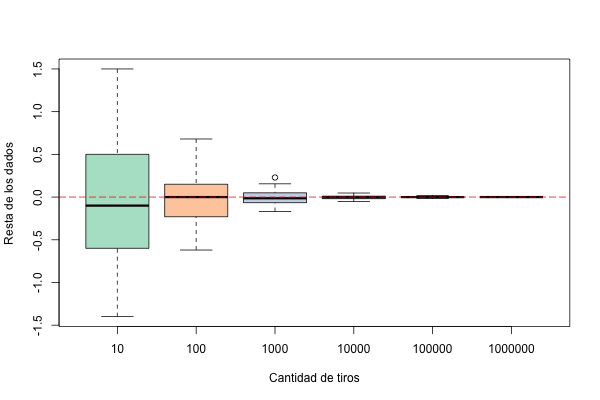
\includegraphics[scale=0.6]{ej2b.png} 		
 	 	\caption{Gráficas de caja con las medias de la resta de dados del ejercicio 2.} 
 	 		\label{ej2b}
\end{figure}
Por último se estima el valor esperado de la variable $XY$, lo cual se automatiza con la función \texttt{dado\_multiplicacion}.
\begin{lstlisting}
dado_multiplicacion <- function(n){
    m <- c()
    for (j in 1:n){
    dado1 <- sample(x = 1:6,size = 1,replace = TRUE)
    dado2 <- sample(x = 1:6,size = 1,replace = TRUE)
    dado <- dado1^2-dado2^2
    m[j] <- dado
    }
return(mean(m))
}
\end{lstlisting}
La figura \ref{ej2c} muestra los gráficos de caja obtenidos, donde se puede apreciar que a mayor valor de \texttt{t} la media se aproxima a 0, el cual es el valor encontrado analíticamente.
\begin{figure}
 	\centering 
 		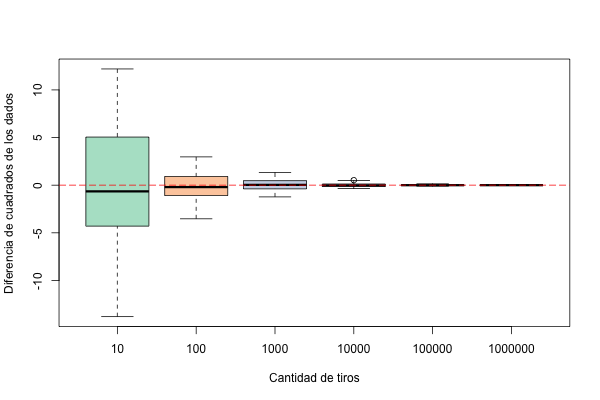
\includegraphics[scale=0.6]{ej2c.png} 		
 	 	\caption{Gráficas de caja con las medias de la multiplicación de dados del ejercicio 2.} 
 	 		\label{ej2c}
\end{figure}

\end{proof}


\begin{ej}[Ej. 15, p.249]
Una caja contiene dos balones dorados y tres plateados. Se te permite tomar sucesivamente balones de la caja al azar. Ganas un dólar cada vez que tomas un balón dorado y pierdes un dólar cada vez que tomas un balón plateado. Después de tomar, el balón no es reemplazado. Demuestra que, si tomas hasta que estás por delante por un dólar o hasta que no hay más balones dorados, este es un juego favorable.
\end{ej}

\begin{proof}[Simulación] 
Para simular este comportamiento del juego se utiliza la función \texttt{balones}, en la cual se representa los balones dorados con 1, ya que es la ganancia que se obtiene al sacar dicho balón y del mismo modo, se representa con 1 a la extracción de un balón plateado.

En la figura \ref{ej3} se muestran las medias obtenidas al aumentar las réplicas del experimento. Como se aprecia en dicha figura, entre mayor número de réplicas la media se aproxima al valor de 0.2 que es el que se obtuvo analíticamente.
\begin{lstlisting}
balones <- function(n) {
    gan <- c() 
    for(j in 1:n){
        ganancia=0
        dorados=0
        balon<-sample(c(1,1,-1,-1,-1))
        for (i in 1:5){
            if(balon[1]==1){
                ganancia<-1
                break

            }
            ganancia=ganancia+balon[i]
            if(balon[i]==1){
                dorados=dorados+1
            }

            if(ganancia==1){
                break
            }
            if(dorados==2){
                break
            }
        }
         gan[j] <- ganancia 
    }
    return(mean(gan))
}
\end{lstlisting}
\begin{figure}
 	\centering 
 		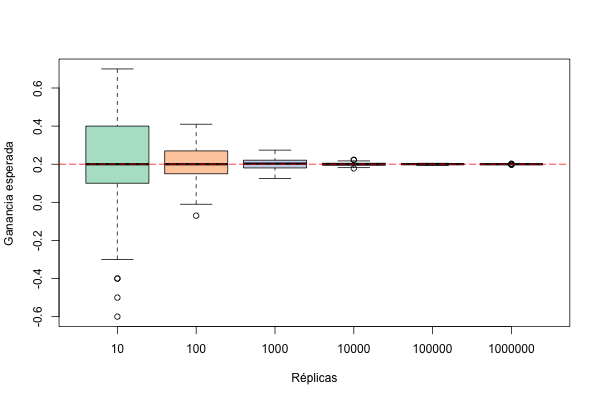
\includegraphics[scale=0.6]{ej3.png} 		
 	 	\caption{Gráficas de caja con las medias del ejercicio 3.} 
 	 		\label{ej3}
\end{figure}
\end{proof}
\begin{ej}[Ej.18, p.249]
Exactamente una de seis llaves similares abre una cierta puerta. Si pruebas las llaves, una después de otra, ¿cuál es el número esperado de llaves que deberá probar antes de tener éxito?.
\end{ej}
\begin{proof}[Simulación] 
Para este ejercicio, se utiliza un ordenamiento pseudo al azar del vector $(1,-1,-1,-1,-1,-1)$, donde la llave que sí abre la puerta se representa con un 1 y las demás con un -1, después se contabilizan los intentos antes del éxito. La función \texttt{llave} guarda los intentos obtenidos en cada iteración y al final regresa la media de dichos intentos. 
\begin{lstlisting}
llave <- function(n) {
    int <- c()
    for (i in 1:n){
        intentos=0
        llaves<-sample(c(1,-1,-1,-1,-1,-1))
        for (j in 1:6){
            if (llaves[j]==1){
                break
            } else {intentos=intentos+1}
   }
    int[i] <- intentos    
        }
    return(mean(int))
}


\end{lstlisting}
En la figura \ref{ej4} se muestran las medias obtenidas al aumentar el número de réplicas, y dichas medias se aproximan al valor 2.5 que es el obtenido de forma analítica. 
\begin{figure}
 	\centering 
 		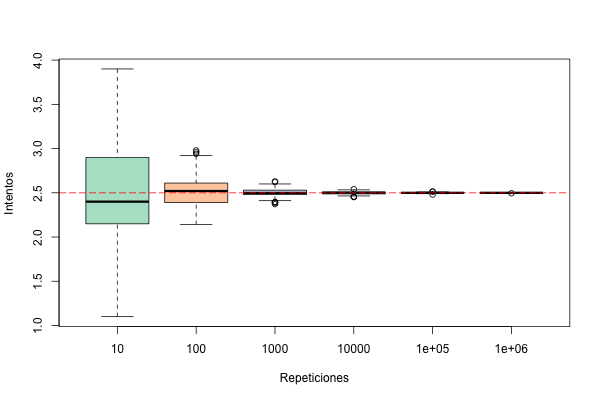
\includegraphics[scale=0.6]{ej4.png} 		
 	 	\caption{Gráficas de caja con las medias del ejercicio 4.} 
 	 		\label{ej4}
\end{figure}
\end{proof}

\begin{ej}[Ej. 19, p.249]
Se tiene un examen de opción múltiple. Un problema tiene cuatro posibles respuestas, y exactamente una es correcta. Se le permite al estudiante escoger un subconjunto de las cuatro posibles respuestas como su respuesta. Si escoge un conjunto que contiene la respuesta correcta, el estudiante recibe tres puntos, pero pierde un punto por cada respuesta incorrecta en el subconjunto escogido. Demuestra que si solo adivina un subconjunto de manera uniforme y aleatoria, su puntuación esperada es cero. 
\end{ej}

\begin{proof}[Simulación] 
Se representa la solución correcta como un 1 y a una solución incorrecta como -1, entonces las posibles respuestas se representa con el vector $(1,-1,-1,-1)$. El estudiante puede elegir 0,1,2,3 o 4 respuestas, entonces se usa \texttt{n} como un número pseudo aleatorio entre 0 y 4 y se eligen \texttt{n} elementos del vector inicial. Si 1 forma parte del subconjunto, gana 3 puntos. Este proceso de elección se automatiza con la función \texttt{examen}, la cual repite el proceso \texttt{k} veces para obtener el promedio del puntaje obtenido.
\begin{lstlisting}
examen <- function(k){
    m <- c()
    for (j in 1:k){
        respuestas <- c(1,-1,-1,-1)
        n <- sample(0:4,1)
        eleccion <- sample(respuestas,n)
        puntaje <- 0
        if (n !=0){
            for (i in 1:n){
                if (eleccion[i]==1){
                    puntaje = puntaje + 3
                } else {puntaje = puntaje - 1}
            }
        }
        m[j] <- puntaje
    }
    return(mean(m))
}
\end{lstlisting}
\begin{figure}
 	\centering 
 		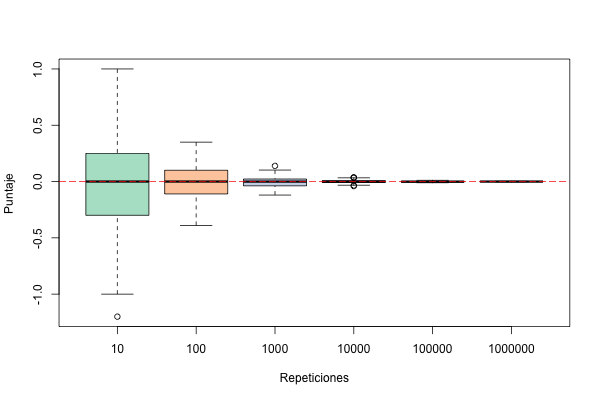
\includegraphics[scale=0.6]{ej5.png} 		
 	 	\caption{Gráficas de caja con las medias del ejercicio 5.} 
 	 		\label{ej5}
\end{figure}
La figura \ref{ej5} muestra las medias obtenidas y como al aumentar el número de repeticiones, la media se aproxima al 0, que es el valor obtenido analíticamente.
\end{proof}


\bibliographystyle{plain} 
\bibliography{ref}


\end{document} 